% Options for packages loaded elsewhere
\PassOptionsToPackage{unicode}{hyperref}
\PassOptionsToPackage{hyphens}{url}
\documentclass[
  10pt,
  a4paper,
]{article}
\usepackage{xcolor}
\usepackage[margin=22mm]{geometry}
\usepackage{amsmath,amssymb}
\setcounter{secnumdepth}{-\maxdimen} % remove section numbering
\usepackage{iftex}
\ifPDFTeX
  \usepackage[T1]{fontenc}
  \usepackage[utf8]{inputenc}
  \usepackage{textcomp} % provide euro and other symbols
\else % if luatex or xetex
  \usepackage{unicode-math} % this also loads fontspec
  \defaultfontfeatures{Scale=MatchLowercase}
  \defaultfontfeatures[\rmfamily]{Ligatures=TeX,Scale=1}
\fi
\usepackage{lmodern}
\ifPDFTeX\else
  % xetex/luatex font selection
\fi
% Use upquote if available, for straight quotes in verbatim environments
\IfFileExists{upquote.sty}{\usepackage{upquote}}{}
\IfFileExists{microtype.sty}{% use microtype if available
  \usepackage[]{microtype}
  \UseMicrotypeSet[protrusion]{basicmath} % disable protrusion for tt fonts
}{}
\makeatletter
\@ifundefined{KOMAClassName}{% if non-KOMA class
  \IfFileExists{parskip.sty}{%
    \usepackage{parskip}
  }{% else
    \setlength{\parindent}{0pt}
    \setlength{\parskip}{6pt plus 2pt minus 1pt}}
}{% if KOMA class
  \KOMAoptions{parskip=half}}
\makeatother
\usepackage{graphicx}
\makeatletter
\newsavebox\pandoc@box
\newcommand*\pandocbounded[1]{% scales image to fit in text height/width
  \sbox\pandoc@box{#1}%
  \Gscale@div\@tempa{\textheight}{\dimexpr\ht\pandoc@box+\dp\pandoc@box\relax}%
  \Gscale@div\@tempb{\linewidth}{\wd\pandoc@box}%
  \ifdim\@tempb\p@<\@tempa\p@\let\@tempa\@tempb\fi% select the smaller of both
  \ifdim\@tempa\p@<\p@\scalebox{\@tempa}{\usebox\pandoc@box}%
  \else\usebox{\pandoc@box}%
  \fi%
}
% Set default figure placement to htbp
\def\fps@figure{htbp}
\makeatother
\setlength{\emergencystretch}{3em} % prevent overfull lines
\providecommand{\tightlist}{%
  \setlength{\itemsep}{0pt}\setlength{\parskip}{0pt}}
\usepackage{mathrsfs}
\newcommand{\Log}{\operatorname{Log}}
\usepackage{mathtools}
\usepackage{xurl}
\emergencystretch=3em
\setcounter{tocdepth}{1}
\newcommand{\Beta}{\mathrm{B}}
\DeclareUnicodeCharacter{00B2}{\ensuremath{^2}}
\DeclareUnicodeCharacter{00B1}{\ensuremath{\pm}}
\DeclareUnicodeCharacter{00D7}{\ensuremath{\times}}
\DeclareUnicodeCharacter{2192}{\ensuremath{\to}}
\DeclareUnicodeCharacter{21D2}{\ensuremath{\Rightarrow}}
\DeclareUnicodeCharacter{21A6}{\ensuremath{\mapsto}}
\DeclareUnicodeCharacter{2208}{\ensuremath{\in}}
\DeclareUnicodeCharacter{2209}{\ensuremath{\notin}}
\DeclareUnicodeCharacter{2212}{\ensuremath{-}}
\DeclareUnicodeCharacter{2227}{\ensuremath{\wedge}}
\DeclareUnicodeCharacter{2228}{\ensuremath{\vee}}
\DeclareUnicodeCharacter{2260}{\ensuremath{\ne}}
\DeclareUnicodeCharacter{2264}{\ensuremath{\le}}
\DeclareUnicodeCharacter{2265}{\ensuremath{\ge}}
\DeclareUnicodeCharacter{2297}{\ensuremath{\otimes}}
\DeclareUnicodeCharacter{00B3}{\ensuremath{^3}}
\DeclareUnicodeCharacter{2074}{\ensuremath{^4}}
\DeclareUnicodeCharacter{2076}{\ensuremath{^6}}
\DeclareUnicodeCharacter{03BB}{\ensuremath{\lambda}}
\DeclareUnicodeCharacter{03BC}{\ensuremath{\mu}}
\DeclareUnicodeCharacter{03B5}{\ensuremath{\epsilon}}
\DeclareUnicodeCharacter{03C4}{\ensuremath{\tau}}
\DeclareUnicodeCharacter{03A6}{\ensuremath{\Phi}}
\DeclareUnicodeCharacter{03B1}{\ensuremath{\alpha}}
\DeclareUnicodeCharacter{03C3}{\ensuremath{\sigma}}
\DeclareUnicodeCharacter{03B4}{\ensuremath{\delta}}
\DeclareUnicodeCharacter{03C0}{\ensuremath{\pi}}
\DeclareUnicodeCharacter{039B}{\ensuremath{\Lambda}}
\DeclareUnicodeCharacter{2202}{\ensuremath{\partial}}
\DeclareUnicodeCharacter{0393}{\ensuremath{\Gamma}}
\DeclareUnicodeCharacter{2205}{\ensuremath{\varnothing}}
\DeclareUnicodeCharacter{221E}{\ensuremath{\infty}}
\DeclareUnicodeCharacter{2200}{\ensuremath{\forall}}
\DeclareUnicodeCharacter{00B9}{\ensuremath{^1}}
\DeclareUnicodeCharacter{00B0}{\ensuremath{{}^\circ}}
\DeclareUnicodeCharacter{211D}{\ensuremath{\mathbb{R}}}
\usepackage{bookmark}
\IfFileExists{xurl.sty}{\usepackage{xurl}}{} % add URL line breaks if available
\urlstyle{same}
\hypersetup{
  hidelinks,
  pdfcreator={LaTeX via pandoc}}

\author{}
\date{}

\begin{document}

{
\setcounter{tocdepth}{3}
\tableofcontents
}
\section{The quarter heat family in the actual ES free-shell
operator}\label{the-quarter-heat-family-in-the-actual-es-free-shell-operator}

23 September 2026. This note transports the quarter family through the
spectral projectors of the actual raw ES operator into its free-shell
carrier. It retains the original forced metric, the full raw matrix
product, the two ordered sheets, all three rotations, every orbit label,
the ambient simplex kernel, and both directed blades. It constructs the
bounded operator on the full orbit Hilbert space, its exact quadratic
algebra receiver and collision pairing, and the full Figure 10
support-corner and modular transport. Every finite orbit compression is
compatible with these maps. No equality with a Weil distribution is
asserted.

The original source read is
\texttt{ES-\allowbreak{}Fable-\allowbreak{}C123/\allowbreak{}es\_\allowbreak{}fable\_\allowbreak{}c123\_\allowbreak{}preprint.\allowbreak{}tex}. The precise inputs
are \texttt{eq:\allowbreak{}raw-\allowbreak{}negative-\allowbreak{}cell-\allowbreak{}projector},
\texttt{eq:\allowbreak{}raw-\allowbreak{}positive-\allowbreak{}cell-\allowbreak{}projector},
\texttt{eq:\allowbreak{}pulled-\allowbreak{}back-\allowbreak{}quarter-\allowbreak{}cell-\allowbreak{}signs},
\texttt{thm:\allowbreak{}quarter-\allowbreak{}three-\allowbreak{}plus-\allowbreak{}one},
\texttt{eq:\allowbreak{}origin-\allowbreak{}resolved-\allowbreak{}support}, \texttt{eq:\allowbreak{}origin-\allowbreak{}involution},
\texttt{eq:\allowbreak{}star-\allowbreak{}kneser-\allowbreak{}D3-\allowbreak{}cover-\allowbreak{}hypotheses},
\texttt{thm:\allowbreak{}general-\allowbreak{}shell-\allowbreak{}123-\allowbreak{}linking-\allowbreak{}decomposition},
\texttt{cor:\allowbreak{}general-\allowbreak{}shell-\allowbreak{}simplex-\allowbreak{}Lorentz-\allowbreak{}pullback}, and
\texttt{thm:\allowbreak{}general-\allowbreak{}shell-\allowbreak{}control-\allowbreak{}determinant-\allowbreak{}volume}. The corresponding
public reading edition is
\href{https://github.com/KokunoYumeto/erdos-straus-foundation/blob/20709bee872ad10e4cc7d7b976d975e24532a803/00_ERDOS_STRAUSS_Project_Reader.pdf}{\emph{Erdős--Straus
Project Reader}, pinned edition 20709bee}. The mathematical reading for
this derivation used the original TeX, not extracted PDF text. All
finite and infinite operator claims below are proved here from the
explicit source matrices and labels.

\subsection{1. The original arithmetic labels and the actual shell
spaces}\label{the-original-arithmetic-labels-and-the-actual-shell-spaces}

For the ES source, let \(p\) be a prime, let \(a_{\rm ar}\) be a
positive integer, and retain \[
R=4a_{\rm ar}-p>2,\qquad\gcd(R,pa_{\rm ar})=1,
\qquad N=pa_{\rm ar}.
\tag{ESHL1}
\] These are \texttt{eq:\allowbreak{}star-\allowbreak{}kneser-\allowbreak{}D3-\allowbreak{}cover-\allowbreak{}hypotheses}. They imply
that \(p\) is odd and \(p\nmid a_{\rm ar}\): for \(p=2\), \(R\) and
\(pa_{\rm ar}\) are both even; for odd \(p\mid a_{\rm ar}\), the same
prime divides \(R\). Define exactly the origin-resolved set \[
\mathcal X_{R,p}=
\{(j,u):j\in\{0,1,2\},\ u\mid a_{\rm ar}^2,
\quad u a_{\rm ar}^{-1}=-p^{1-j}\text{ in }(\mathbb Z/R\mathbb Z)^\times\}.
\tag{ESHL2}
\] All inverses in this formula exist by ESHL1. Its involution is \[
\iota(j,u)=(2-j,a_{\rm ar}^2/u).
\tag{ESHL3}
\] It preserves the defining congruence because taking its
multiplicative inverse turns \(-p^{1-j}\) into \(-p^{j-1}\). Applying it
twice gives the identity. A fixed point would have \(j=1,u=a_{\rm ar}\);
the congruence would then give \(1=-1\pmod R\), impossible for \(R>2\).
Thus all its orbits have size two.

Let \(\mathcal O=\mathcal X_{R,p}/\langle\iota\rangle\) and
\(q=|\mathcal O|\). The two divisors \(d(j,u)=p^ju\) in any orbit have
product \(N^2\). They are unequal: uniqueness of the representation
\(p^ju\), using \(p\nmid a_{\rm ar}\), would otherwise give a fixed
point of \(\iota\). Thus each orbit has a unique low member \(x_O^-\)
with divisor below \(N\) and high member \(x_O^+\) with divisor above
\(N\). This proves the original ordering used by the source.

The complete free-cover labels are \((O,\epsilon,m)\), where
\(\epsilon\in\{0,1\}\) names the low/high sheet and
\(m\in\mathbb Z/3\mathbb Z\) names the rotation. The original bijection
and its unitary linearization are \[
\theta_{123}(m,x_O^\epsilon)=(O,\epsilon,m),
\quad
\Theta_{123}:\mathbb C[\widetilde{\mathcal X}_{R,p}]
\longrightarrow \mathcal H_q:=\mathbb C[\mathcal O]\otimes\mathbb C^2\otimes\mathbb C^3,
\quad e_{(m,x_O^\epsilon)}\mapsto e_O\otimes f_\epsilon\otimes g_m.
\tag{ESHL4}
\] They are bijections because the three labels recover the original
point. The map is unitary for the stated orthonormal label bases. Hence
\(\dim\mathcal H_q=6q\), retaining every label.

Let \(P_2=I_3-\mathbf1\mathbf1^*/3\) be the source triangle support
projector. The original support unitary
\(\mathsf U_2:\operatorname{Ran}P_2\to\mathbb C^2\) satisfies
\(\mathsf U_2^*\mathsf U_2=P_2\) and \(\mathsf U_2\mathsf U_2^*=I_2\),
as proved in \texttt{eq:\allowbreak{}simplex-\allowbreak{}123-\allowbreak{}unitary-\allowbreak{}identities}. Write
\(\eta_\epsilon=\mathsf U_2^*f_\epsilon\). These are an orthonormal
basis of the original triangle support, with their original coordinate
choice retained. The actual ambient simplex space and its support are \[
\mathcal K_q=\mathbb C[\mathcal O]\otimes\mathbb C^3\otimes\mathbb C^3,
\qquad
\mathcal H_q^{\rm simp}=\mathbb C[\mathcal O]\otimes\operatorname{Ran}P_2\otimes\mathbb C^3.
\tag{ESHL5}
\] The isometry \(V_q=I\otimes\mathsf U_2^*\otimes I_3\) identifies
\(\mathcal H_q\) with \(\mathcal H_q^{\rm simp}\). Its range projector
is \(P_q^{\rm simp}=I\otimes P_2\otimes I_3\). The retained
complementary space is \[
\mathcal Z_q=\mathbb C[\mathcal O]\otimes\mathbb C\mathbf1\otimes\mathbb C^3,
\quad\mathcal K_q=\mathcal H_q^{\rm simp}\oplus\mathcal Z_q,
\quad\dim\mathcal Z_q=3q.
\tag{ESHL6}
\] This ambient kernel is different from the source map \(\Pi_{123}\),
which sends all six labels in an orbit to one support label and has
kernel dimension \(5q\). Explicitly that latter kernel is the subspace
whose six coefficients sum to zero on every orbit. Neither of these
kernels is substituted for the other.

\subsection{2. The raw quarter operator and its spectral
algebra}\label{the-raw-quarter-operator-and-its-spectral-algebra}

Give the raw four-cell vector space
\(\mathcal V_{\rm raw}=M_2(\mathbb C)\) its Hilbert--Schmidt inner
product, with orthonormal basis \(E_{11},E_{12},E_{21},E_{22}\). The
original forced ES metric is retained by the explicit isometry
ESHL43--ESHL44 below. The source's pulled-back quarter reflection acts
by \[
\mathfrak Q_\square(E_{11})=E_{11},\quad
\mathfrak Q_\square(E_{12})=E_{12},\quad
\mathfrak Q_\square(E_{21})=-E_{21},\quad
\mathfrak Q_\square(E_{22})=E_{22}.
\tag{ESHL7}
\] Consequently its orthogonal spectral projectors are \[
P_-(M)=M_{21}E_{21},\qquad P_+=I_{\mathcal V_{\rm raw}}-P_-.
\tag{ESHL8}
\] They satisfy \(P_\pm^2=P_\pm=P_\pm^*\), \(P_+P_-=0\), with ranks
three and one. Define the exact raw quarter operator and its heat family
by \[
A_0=\tfrac14P_+-\tfrac14P_-,\qquad
A_h=\tfrac14P_++a(h)P_-,\qquad a(h)=-\tfrac14+2h.
\tag{ESHL9}
\] The original coefficient inversion matrix \(\mathcal I_-\) is
transported to this raw presentation by the source map
\(\mathcal T_\square\), since \texttt{eq:\allowbreak{}pulled-\allowbreak{}back-\allowbreak{}quarter-\allowbreak{}reflection}
states
\(\mathfrak Q_\square=\mathcal T_\square^{-1}(4\mathcal I_-)\mathcal T_\square\).
Thus \(A_0\) is the actual pulled-back quarter operator.

The fixed spectral algebra is \[
\mathcal D=\mathbb C[A_0]
=\{cP_++dP_-:c,d\in\mathbb C\}\cong\mathbb C^2.
\tag{ESHL10}
\] Indeed \(P_+=2A_0+I/2\), \(P_-=-2A_0+I/2\), so both projectors belong
to the generated algebra. Their orthogonality proves multiplication is
coordinatewise and the involution conjugates \(c,d\). The representation
is faithful because both projectors have nonzero range.

The original forced metric in \texttt{eq:\allowbreak{}Fable-\allowbreak{}forced-\allowbreak{}full-\allowbreak{}metric}, also
used in ESQ9, has matrix \[
G=\begin{pmatrix}
1/16&0&0&-7/144\\
0&2/9&0&0\\
0&0&1&0\\
-7/144&0&0&1/16
\end{pmatrix}.
\tag{ESHL43}
\] Let \(v_+=(E_{11}+E_{22})/\sqrt2\), \(v_-=(E_{11}-E_{22})/\sqrt2\),
and let \(\Pi_+,\Pi_-,\Pi_{12},\Pi_{21}\) be the Hilbert--Schmidt
projections on these two unit vectors and on \(E_{12},E_{21}\),
respectively. Multiplying ESHL43 by these four vectors gives the
respective eigenvalues \(1/72,1/9,2/9,1\). Hence the fully specified
positive square root is \[
T=G^{1/2}=\frac1{6\sqrt2}\Pi_++\frac13\Pi_-
 +\frac{\sqrt2}{3}\Pi_{12}+\Pi_{21},\qquad
T^*T=G,\qquad TP_\pm=P_\pm T,\qquad TA_h=A_hT.
\tag{ESHL44}
\] The four orthogonal projections sum to the identity. Squaring their
positive coefficients proves \(T^*T=G\), and replacing the coefficients
by their reciprocals defines the inverse. Each projection preserves the
decomposition into \(\operatorname{Ran}P_+\) and
\(\operatorname{Ran}P_-\), proving both commutation identities. Thus
\(T:(\mathcal V_{\rm raw},\langle x,Gy\rangle_{\rm HS})\to(\mathcal V_{\rm raw},\langle x,y\rangle_{\rm HS})\)
is an isometry, and the original heat form is exactly
\(\langle x,GA_hy\rangle_{\rm HS}=\langle Tx,A_hTy\rangle_{\rm HS}\).
Conjugation by \(T\) fixes every member of the spectral algebra
\(\mathcal D\). This is a vector-metric transport, and does not change
the raw matrix product: for example \(T(I_2)=I_2/(6\sqrt2)\), so \(T\)
is not a unital algebra map. The separate map preserving that product is
ESHL45.

The spectral algebra \(\mathcal D\) consists of endomorphisms of the raw
four-cell vector space. Its negative projector is the two-sided corner
operation \(P_-(X)=E_{22}XE_{11}\), as direct entry multiplication
proves. It is not a left multiplication operator: \(P_-\) has rank one,
whereas left multiplication by a nonzero rank-one matrix on
\(M_2(\mathbb C)\) has rank two, since each of two columns independently
ranges over a fixed one-dimensional image. Section 3 uses the spectral
algebra as its domain; ESHL45--ESHL47 construct the full raw matrix
algebra map and intertwine this corner operation exactly.

\subsection{3. The faithful spectral lift into the actual ordered
sheets}\label{the-faithful-spectral-lift-into-the-actual-ordered-sheets}

In \(\mathcal H_q\), define the original low and high projectors \[
Q_<=I_{\mathbb C[\mathcal O]}\otimes E_{11}^{(2)}\otimes I_3,
\qquad Q_>=I_{\mathbb C[\mathcal O]}\otimes E_{22}^{(2)}\otimes I_3.
\tag{ESHL11}
\] They are exactly \texttt{eq:\allowbreak{}general-\allowbreak{}shell-\allowbreak{}ordered-\allowbreak{}sheet-\allowbreak{}projectors}
under ESHL4. Their ranges are orthogonal, they sum to the identity on
\(\mathcal H_q\), and each has dimension \(3q\). For \(q\ge1\), define
\[
\boxed{\Psi_q:\mathcal D\longrightarrow B(\mathcal H_q),
\qquad cP_++dP_-\longmapsto cQ_<+dQ_>.}
\tag{ESHL12}
\] This is a faithful unital \(*\)-homomorphism. Orthogonality gives
\((cQ_<+dQ_>)(c'Q_<+d'Q_>)=cc'Q_<+dd'Q_>\), matching the source product.
Adjoints conjugate the same two coefficients. The source unit maps to
\(Q_<+Q_>=I\). If an image vanishes, applying it to any low and any high
basis vector gives \(c=d=0\). This proves faithfulness and also the
isometry \(\|\Psi_q(cP_++dP_-)\|=\max(|c|,|d|)\).

The map retains the two spectral labels, but changes their
representation multiplicities. Its exact trace comparison is \[
\operatorname{Tr}_{\rm raw}(cP_++dP_-)=3c+d,
\qquad \operatorname{Tr}_{\mathcal H_q}\Psi_q(cP_++dP_-)=3q(c+d).
\tag{ESHL13}
\] Thus this is not a trace-preserving or Hilbert-space unitary
identification of the four-cell space with the shell. Both multiplicity
lists remain explicit. When \(q=0\), the shell space and all its
operators are zero; the resulting map is zero and is not faithful. The
nonzero-shell assertion has therefore not been extended to an empty
arithmetic shell.

Define the fixed positive weight and its inverse on the support by \[
W=16Q_<+4Q_>,\qquad W^{-1}=\tfrac1{16}Q_<+\tfrac14Q_>.
\tag{ESHL14}
\] Both are verified by multiplication. The weight commutes with
\(\Psi_q(\mathcal D)\), and its positive square root is \(4Q_<+2Q_>\).
The lifted heat carrier is \[
\boxed{H_h:=W\Psi_q(A_h)=4Q_<+t(h)Q_>,
\qquad t(h)=-1+8h.}
\tag{ESHL15}
\] At zero it equals the actual ES carrier \[
H_0=I_{\mathbb C[\mathcal O]}\otimes\operatorname{diag}(4,-1)\otimes I_3
=H^{\rm sh}_{R,p},
\tag{ESHL16}
\] in the source's unitary presentation
\texttt{eq:\allowbreak{}general-\allowbreak{}shell-\allowbreak{}restricted-\allowbreak{}Lorentz-\allowbreak{}carrier}. The map
\(A\mapsto W\Psi_q(A)\) is a specified positive linear map on
self-adjoint elements, since it also equals \(W^{1/2}\Psi_q(A)W^{1/2}\);
it is not asserted to be an algebra homomorphism. The faithful
homomorphism is \(\Psi_q\) itself.

The original simplex presentation is \(\widetilde H_h=V_qH_hV_q^*\) on
\(\mathcal K_q\), with zero action on \(\mathcal Z_q\). This gives the
exact commuting relation \(\widetilde H_hV_q=V_qH_h\), and the
support-corner homomorphism \(D\mapsto V_q\Psi_q(D)V_q^*\) has unit
\(P_q^{\rm simp}\). It is unital as a map to that corner, not to the
whole ambient algebra with identity \(I_{\mathcal K_q}\).

\subsection{4. Positivity, the sharp gap, and every
kernel}\label{positivity-the-sharp-gap-and-every-kernel}

For \(x=x_<+x_>\) in the orthogonal sheet decomposition, \[
\langle x,H_hx\rangle=4\|x_<\|^2+t(h)\|x_>\|^2.
\tag{ESHL17}
\] Thus for a nonempty finite shell \[
\operatorname{inertia}(H_h)=
\begin{cases}
(3q,3q,0),&h<1/8,\\
(3q,0,3q),&h=1/8,\\
(6q,0,0),&h>1/8.
\end{cases}
\tag{ESHL18}
\] In particular \(H_h\succeq0\) exactly for \(h\ge1/8\). For \(h>1/8\),
the sharp lower and upper bounds are \[
\boxed{\min(4,-1+8h)I\preceq H_h
\preceq\max(4,-1+8h)I.}
\tag{ESHL19}
\] Both constants are attained on the appropriate sheet vectors in
ESHL17. The lower bound is independent of \(q\). At the critical time,
the kernel on the shell is exactly \(\operatorname{Ran}Q_>\).

On the full simplex ambient space, the kernel is \(\mathcal Z_q\) for
\(h\ne1/8\), and is \[
\ker\widetilde H_{1/8}=\mathcal Z_q\oplus V_q\operatorname{Ran}Q_>,
\quad\dim\ker\widetilde H_{1/8}=6q.
\tag{ESHL20}
\] The original ambient kernel has not disappeared when the support form
becomes positive. The sharp lower bound on the ambient space is the
support inequality \(\widetilde H_h\succeq\min(4,t(h))P_q^{\rm simp}\)
for \(h>1/8\); strict positivity is a statement on
\(\mathcal H_q^{\rm simp}\).

There are also two distinct times at which a single operator loses its
ability to recover the fixed spectral labels. At \(h=1/4\), \(A_h=I/4\),
so \(\mathbb C[A_h]=\mathbb CI\) although the fixed algebra
\(\mathcal D\) and its \(P_\pm\) remain. At \(h=5/8\), \(H_h=4I\), so
its generated algebra is scalar although \(Q_<,Q_>\) remain present.
These follow by equating their two coefficients. The lift uses
\(\mathcal D=\mathbb C[A_0]\) and the retained labelled projectors
throughout; it does not reconstruct them from the possibly scalar single
operator at these times.

\subsection{5. The actual mixed blades remain
nonzero}\label{the-actual-mixed-blades-remain-nonzero}

Retain exactly the directed blades of
\texttt{eq:\allowbreak{}general-\allowbreak{}shell-\allowbreak{}low-\allowbreak{}high-\allowbreak{}blade-\allowbreak{}transport} and
\texttt{eq:\allowbreak{}general-\allowbreak{}shell-\allowbreak{}high-\allowbreak{}low-\allowbreak{}blade-\allowbreak{}transport}: \[
D=I\otimes2E_{21}^{(2)}\otimes I_3,
\qquad U=I\otimes2E_{12}^{(2)}\otimes I_3=D^*.
\tag{ESHL21}
\] Here \(D\) is the original low-to-high sheet map and \(U\) its
adjoint; these symbols do not denote the amplitude multiplier from a
different packet calculation. Matrix-unit multiplication proves \[
D^2=U^2=0,\qquad UD=4Q_<,\qquad DU=4Q_>,
\quad\|D\|=\|U\|=2.
\tag{ESHL22}
\] Their norms follow because each takes a unit vector in its source
sheet to a vector of norm two and kills the other sheet. They are
nonzero for \(q\ge1\), at every heat time. Their precise source and
target spaces are \[
D:\operatorname{Ran}Q_<\to\operatorname{Ran}Q_>,
\qquad U:\operatorname{Ran}Q_>\to\operatorname{Ran}Q_<.
\tag{ESHL23}
\] The carrier consequently retains the original directed expression \[
H_h=UD+t(h)Q_>.
\tag{ESHL24}
\] At \(h=0\), this is exactly
\texttt{eq:\allowbreak{}general-\allowbreak{}shell-\allowbreak{}directed-\allowbreak{}Gram-\allowbreak{}support-\allowbreak{}carrier}. At \(h=1/8\),
the high sheet becomes the carrier's kernel, but \(D\) still takes the
positive sheet onto that kernel and \(U\) takes it back. The commutators
are \[
[H_h,D]=(t(h)-4)D,\qquad [H_h,U]=(4-t(h))U.
\tag{ESHL25}
\] Both follow by multiplying the two diagonal coefficients with the two
matrix units. Thus the mixed maps have not been discarded by
diagonalizing the form.

Their generated algebra is exactly \[
I_{\mathbb C[\mathcal O]}\otimes M_2(\mathbb C)\otimes I_3:
\quad E_{11}\mapsto Q_<,\ E_{22}\mapsto Q_>,
\ E_{21}\mapsto D/2,\ E_{12}\mapsto U/2.
\tag{ESHL26}
\] The four matrix-unit laws hold by ESHL22 and the sheet actions;
independence follows by applying a proposed relation to one low and one
high vector. This is an actual copy of the raw matrix algebra
\(M_2(\mathbb C)\), with its diagonal subalgebra containing
\(\Psi_q(\mathcal D)\). The faithful algebra isomorphism onto this image
is \(R_q\) in ESHL45. Section 2 identifies the spectral projector
\(P_-\) with a two-sided corner operation on that algebra; it does not
exclude the matrix algebra identification.

There is a faithful dual-number receiver
\(\mathbb C[\eta]/\eta^2\to B(\mathcal H_q)\), \(1\mapsto I\),
\(\eta\mapsto D\). Its multiplicativity follows from \(D^2=0\); applying
\(cI+dD=0\) first to a high vector and then to a low vector proves
injectivity. These nilpotents are present in the mixed operator algebra
at all times. The diagonal homomorphism \(\Psi_q\) does not itself
create a nilpotent in its reduced domain \(\mathbb C^2\).

The original rotation acts only on the third factor and commutes with
\(D,U,H_h\). The original reflection swaps the two sheet factors and
reverses rotation labels, giving \[
\mathbf S D\mathbf S^{-1}=U,
\quad\mathbf S Q_<\mathbf S^{-1}=Q_>,
\quad\mathbf S H_h\mathbf S^{-1}=t(h)Q_<+4Q_>.
\tag{ESHL27}
\] These follow directly from the source label action in
\texttt{eq:\allowbreak{}general-\allowbreak{}shell-\allowbreak{}123-\allowbreak{}label-\allowbreak{}action}. The directed carrier is
invariant under that reflection only when \(t(h)=4\). Its exact
reflected partner, rather than an unproved invariance, is retained in
ESHL27.

\subsection{6. Exact finite traces, lengths, and determinant
ratios}\label{exact-finite-traces-lengths-and-determinant-ratios}

For finite \(q\ge1\), the two eigenvalues and their multiplicities give
\[
\operatorname{Tr}H_h=3q(4+t),\quad
\|H_h\|_{\rm HS}^2=3q(16+t^2),\quad
\det H_h=4^{3q}t^{3q},
\quad t=-1+8h.
\tag{ESHL28}
\] The Hilbert--Schmidt formula is the trace of the square because
\(H_h\) is Hermitian. The determinant is the product of all eigenvalues,
including its sign. For \(t\ne0\), its absolute determinant volume and
the exact ratio to the original carrier are \[
V_h^{\det}=|4t|^{3q},\qquad
\frac{V_h^{\det}}{V_0^{\det}}=|t|^{3q},
\qquad \det(H_hH_0^{-1})=(-t)^{3q}=(1-8h)^{3q}.
\tag{ESHL29}
\] The last formula follows also from \(H_hH_0^{-1}=Q_<-tQ_>\). At the
critical time the determinant is zero; no logarithm of that zero is
treated as finite.

The exact traceless part is \[
K_h=H_h-\frac{4+t}{2}I
=\frac{4-t}{2}(Q_<-Q_>),
\qquad \|K_h\|_{\rm HS}^2=\frac{3q}{2}(4-t)^2.
\tag{ESHL30}
\] For the constant-generator paths \(\exp(-i\sigma H_h)\),
\(\exp(-i\sigma K_h)\), \(0\le\sigma\le1\), the Hilbert--Schmidt speed
is the norm of the generator: multiplying the derivative by the inverse
unitary removes the unitary factor and leaves the same Hilbert--Schmidt
norm. Thus their squared lengths equal the two squared norms in ESHL28
and ESHL30. At \(h=0\) they are \(51q\) and \(75q/2\), exactly the ES
source constants.

All per-orbit quantities have exact finite formulas, with the full
factor \(q\) retained: \[
\frac{\operatorname{Tr}H_h}{q}=3(4+t),\quad
\frac{\|H_h\|_{\rm HS}^2}{q}=3(16+t^2),\quad
\frac{\log V_h^{\det}}q=3\log|4t|\quad(t\ne0).
\tag{ESHL31}
\] For \(t\ne0\), these imply \[
\log V_h^{\det}
=\frac{\log|4t|}{16+t^2}\|H_h\|_{\rm HS}^2.
\tag{ESHL32}
\] For \(t\ne0,4\), they also imply \[
\log V_h^{\det}
=\frac{2\log|4t|}{(4-t)^2}\|K_h\|_{\rm HS}^2.
\tag{ESHL33}
\] At \(t=-1\), these coefficients are \(2\log2/17\) and \(4\log2/25\),
reproducing the original determinant-length identities. At \(t=4\),
\(K_h=0\) while \(V_h^{\det}=16^{3q}\), so the second quotient is not
defined; the original exact formulas still apply. This handles the
exceptional scalar carrier explicitly.

\subsection{7. The actual infinite orbit-space
operator}\label{the-actual-infinite-orbit-space-operator}

Let \(\mathcal O_\infty\) be any nonempty countable set of the retained
labelled complement orbits, with shell labels included when orbits from
different shells are combined. The empty case is the zero space already
specified after ESHL13. Form the actual Hilbert completion \[
\mathcal H_\infty=\ell^2(\mathcal O_\infty)\otimes\mathbb C^2\otimes\mathbb C^3.
\tag{ESHL34}
\] This definition also covers a finite orbit set. If it is infinite,
the following statements concern that same labelled Hilbert space; no
assertion that every arithmetic shell is occupied is being introduced.
The projectors \(Q_<,Q_>\), blades \(D,U\), weight \(W\), and
\(\Psi_\infty\) are defined by the identical tensor formulas
ESHL11--ESHL15 and ESHL21.

For example, if \(x=(x_{O,<,m},x_{O,>,m})\), then \[
(H_hx)_{O,<,m}=4x_{O,<,m},\qquad
(H_hx)_{O,>,m}=t(h)x_{O,>,m}.
\tag{ESHL35}
\] The square sum of these coordinates is bounded by
\(\max(16,t(h)^2)\|x\|^2\), proving that \(H_h\) is everywhere defined
and bounded. Choosing a single sheet basis vector proves \[
\|H_h\|=\max(4,|t(h)|),\qquad
\|H_h-H_{h'}\|=8|h-h'|.
\tag{ESHL36}
\] Its adjoint is itself by the real diagonal coefficients. Its
quadratic form is the convergent sum of ESHL17 over all labels, so the
positivity criterion and sharp uniform lower bound ESHL19 remain valid
without a dimension-dependent error. In particular, for every fixed
\(h>1/8\), \(H_h\) is boundedly invertible on the entire orbit support,
with \[
H_h^{-1}=\tfrac14Q_<+\frac1{t(h)}Q_>,
\qquad\|H_h^{-1}\|=\frac1{\min(4,t(h))}.
\tag{ESHL37}
\] This is an explicit inverse, verified by multiplication. At
\(h=1/8\), its kernel is the whole high-sheet Hilbert subspace and its
range is the low-sheet subspace. The blades remain bounded with norm two
and retain every identity ESHL22--ESHL27.

The infinite ambient simplex space is
\(\mathcal K_\infty=\ell^2(\mathcal O_\infty)\otimes\mathbb C^3\otimes\mathbb C^3\).
Its orthogonal decomposition is the completed version of ESHL5--ESHL6,
and \(V_\infty=I\otimes\mathsf U_2^*\otimes I_3\) gives the same
isometry and support projector. The zero action on the entire
complementary Hilbert space is retained, including when \(H_h\) is
uniformly positive on its support.

For completeness, every local matrix unit also remains an actual bounded
operator. For basis labels \(\alpha=(O,\epsilon,m)\),
\(\beta=(O',\epsilon',m')\), define \[
E_{\alpha\beta}x=e_\alpha\langle e_\beta,x\rangle.
\tag{ESHL38}
\] Its norm is one, its adjoint is \(E_{\beta\alpha}\), and
\(E_{\alpha\beta}E_{\gamma\delta}=\delta_{\beta\gamma}E_{\alpha\delta}\),
all by direct application to a vector. Thus the mixed maps, including
maps between different orbit labels, are present in
\(B(\mathcal H_\infty)\). The particular global blades are the strong
sums \(D=2\sum_{O,m}E_{(O,>,m),(O,<,m)}\) and its adjoint, whose
orthogonal source and target coordinates give norm two.

\subsection{8. Exact compatibility with all finite
compressions}\label{exact-compatibility-with-all-finite-compressions}

For a finite subset \(F\subset\mathcal O_\infty\), take all two-sheet
and three-rotation labels over its orbits. Let
\(j_F:\mathcal H_F\to\mathcal H_\infty\) be inclusion by zero outside
\(F\), and \(P_F=j_Fj_F^*\). It is an isometry. The tensor formulas give
\[
H_hj_F=j_FH_{h,F},\quad j_F^*H_hj_F=H_{h,F},
\quad P_FH_h=H_hP_F,
\quad\Psi_\infty(A)j_F=j_F\Psi_F(A).
\tag{ESHL39}
\] The same equations hold for \(D,U,W\) and the original rotation and
reflection operators because none changes the orbit label. Thus these
are the actual finite lifts and their exact inclusions, not new finite
approximations with altered sheets or rotations.

For nested finite orbit sets \(F_n\) exhausting \(\mathcal O_\infty\),
the square-summable tail identity gives \(\|(I-P_{F_n})x\|\to0\) for
every \(x\). Therefore \[
P_{F_n}H_hP_{F_n}\longrightarrow H_h
\quad\text{strongly on }\mathcal H_\infty.
\tag{ESHL40}
\] Indeed the difference on \(x\) has norm at most
\(\|H_h\|\|(I-P_{F_n})x\|\), since the projections commute with \(H_h\).
Positivity and its uniform bound already hold on every finite
compression and on the limiting operator by ESHL17; there is no hidden
loss of the lower bound in this limit. If every \(F_n\) has a nonempty
complement, this convergence is not in operator norm: a unit tail vector
in a sheet attaining the maximum eigenvalue magnitude has difference
norm \(\max(4,|t(h)|)\). The exact topology of convergence is thereby
specified.

\subsection{9. Infinite traces and the retained finite-volume
data}\label{infinite-traces-and-the-retained-finite-volume-data}

When \(\mathcal O_\infty\) is infinite, \(H_h\) is never
Hilbert--Schmidt: its value on each of infinitely many low-sheet basis
vectors has norm four, so the sum of their squared norms diverges. It is
not trace class for the same reason, since \(|H_h|\) has eigenvalue four
infinitely often. For \(h\ge1/8\), its extended positive trace is
\(+\infty\). For \(h<1/8\), its positive and negative parts both have
infinite trace, so an ordinary signed trace would be the undefined
difference \(\infty-\infty\). None of these facts changes its bounded
operator norm or the positive lower bound at \(h>1/8\).

The ordinary finite-dimensional determinant has no direct
infinite-dimensional value here. More precisely, for \(h\ne0\), the
relative operator is \[
H_hH_0^{-1}=I-8hQ_>.
\tag{ESHL41}
\] Its difference from the identity is not compact: it takes an infinite
orthonormal sequence in the high sheet to an orthogonal sequence of
fixed nonzero norm. Hence that difference is not trace class, and the
usual trace-class Fredholm determinant is unavailable. At \(h=0\) the
relative operator is the identity and its determinant is one.

The exact finite determinants and per-orbit data remain ESHL28--ESHL33
on every finite subset. Their absolute values can tend to zero,
infinity, or remain one, depending on \(|4t(h)|\); none of those
sequence behaviours alone defines an ordinary determinant of the
infinite operator. On the specified constant-fibre algebra
\(I_{\ell^2(\mathcal O_\infty)}\otimes M_6(\mathbb C)\), there is
instead the exact finite fibre trace
\(\tau_{\rm fibre}(I\otimes B)=\operatorname{Tr}_{\mathbb C^6}B\). It
equals \(\operatorname{Tr}_{\mathcal H_F}(j_F^*(I\otimes B)j_F)/|F|\) on
every nonempty finite orbit set. Thus, for \(t(h)\ne0\), the explicitly
defined fibre determinant is \[
\exp\bigl(\tau_{\rm fibre}(\log|H_h|)\bigr)=|4t(h)|^3.
\tag{ESHL42}
\] This is a finite-fibre observable with its exact comparison map; it
is not presented as an ordinary infinite determinant. The full orbit
labels, all local injections, the fixed spectral representation, and the
ambient kernel remain in the construction.

The result is a lift of the stated quarter heat family into the actual
ES free-shell carrier, with a bounded infinite-orbit extension and a
uniform positive support bound after \(h=1/8\). The full raw
multiplication and quadratic receiver are constructed in ESHL45--ESHL50,
the collision pairing in ESHL51--ESHL53, and the complete Figure 10
transport in ESHL54--ESHL64. These maps do not identify the ES spectral
algebra or its infinite orbit trace with an arithmetic Weil pairing.

\subsection{10. Exact finite
verification}\label{exact-finite-verification}

The reproducible script \texttt{check\_\allowbreak{}es\_\allowbreak{}shell\_\allowbreak{}heat\_\allowbreak{}lift.\allowbreak{}py} passed
\textbf{217 exact symbolic checks}, recorded in
\texttt{ES\_\allowbreak{}SHELL\_\allowbreak{}HEAT\_\allowbreak{}LIFT\_\allowbreak{}CHECKS.\allowbreak{}json}. They verify the raw
spectral projectors and their multiplicities, the original forced metric
isometry, the full raw matrix product and corner operation, the
quadratic receiver and its original involution, the complete collision
pairing, both blade products and nilpotence, all stated trace and
determinant formulas, the original control-length constants, and the
ambient kernel dimensions for one, two, and three complete orbit blocks.
They also check finite inclusions retaining all six labels per orbit;
the original displayed segment, triangle, and tetrahedron synthesis
matrices; all nine rectangular corners and their 27 typed compositions;
all 36 density ratios; the full Hilbert--Schmidt map; inter-orbit
transport; and the exact ambient multiplicativity defect. The bounded
infinite extension, its sharp lower bound, and strong convergence are
proved in ESHL34--ESHL40 and ESHL62--ESHL63; they are not inferred from
the finite checks.

\subsection{11. The full raw matrix product and its exact corner
operation}\label{the-full-raw-matrix-product-and-its-exact-corner-operation}

For every nonempty finite or countable orbit set \(\mathcal O\), use its
Hilbert space
\(\mathcal H_{\mathcal O}=\ell^2(\mathcal O)\otimes\mathbb C^2\otimes\mathbb C^3\),
where \(\ell^2(\mathcal O)=\mathbb C[\mathcal O]\) when the set is
finite. Define \[
R_{\mathcal O}:M_2(\mathbb C)\longrightarrow B(\mathcal H_{\mathcal O}),
\qquad R_{\mathcal O}(X)=I_{\ell^2(\mathcal O)}\otimes X\otimes I_3.
\tag{ESHL45}
\] The tensor product laws give \(R(XY)=R(X)R(Y)\), \(R(I_2)=I\), and
\(R(X^*)=R(X)^*\). If \(R(X)=0\), fix an orbit \(O\) and rotation \(m\);
its restriction to the span of
\(e_O\otimes f_0\otimes g_m,e_O\otimes f_1\otimes g_m\) is the matrix
\(X\), so \(X=0\). This proves faithfulness. The same restriction,
together with the square-sum norm bound over all \((O,m)\), proves
\(\|R(X)\|=\|X\|\). The inverse on its image is precisely that
two-dimensional restriction for any fixed \((O,m)\), independent of the
choice. Its image is the whole blade algebra ESHL26, since it sends
\(E_{11},E_{22},E_{21},E_{12}\) to \(Q_<,Q_>,D/2,U/2\), respectively.

Entry multiplication in the original raw matrix algebra gives
\(P_-(X)=E_{22}XE_{11}\). Applying the multiplicative map just proved
gives \[
R(P_-X)=Q_>R(X)Q_<,
\qquad
R(A_hX)=\frac14R(X)+\left(a(h)-\frac14\right)Q_>R(X)Q_<.
\tag{ESHL46}
\] Thus the quarter operator acts on the blade algebra by the explicitly
displayed linear operation on operators. This is the exact relation
between the spectral endomorphism and the matrix multiplication. It is
different from left multiplication by the heat carrier \(H_h\): the
former fixes the upper-right matrix cell with coefficient \(1/4\), while
\(H_hR(E_{12})=4R(E_{12})\). Both actions are retained with their
domains and constants. The spectral lift \(\Psi(A_h)\) of ESHL12 and the
operator-valued map \(X\mapsto R(A_hX)\) of ESHL46 also have different
domains; ESHL46 is their explicitly calculated underlying raw-cell
action, not an asserted equality of those maps.

For finite \(q\), the matrix trace on \(q\) identical orbit blocks and
three identical rotation blocks gives \[
\operatorname{Tr}(R(X)^*R(Y))=3q\operatorname{tr}_2(X^*Y),
\qquad
\operatorname{Tr}(R(TX)^*R(TY))=3q\langle X,GY\rangle_{\rm HS}.
\tag{ESHL47}
\] The second equality follows from the first and \(T^*T=G\); \(TX\)
means the four-dimensional linear metric map ESHL44 applied to the raw
matrix viewed as a vector. If \(\widehat A_h\) denotes the linear
operator in the right side of ESHL46, then
\(\widehat A_hR(TY)=R(A_hTY)=R(TA_hY)\). Inserting this in ESHL47 gives
\(\operatorname{Tr}(R(TX)^*\widehat A_hR(TY))=3q\langle X,GA_hY\rangle_{\rm HS}\).
This proves the original metric and form transport alongside the
product-preserving map. For an infinite orbit set, the same formulas
with the finite fibre trace \(\tau_{\rm fibre}\) replace \(3q\) by
\(3\); the ordinary traces of these repeated operators need not be
finite.

\subsection{12. The original quadratic algebra, its involution, and the
vanishing
infinitesimal}\label{the-original-quadratic-algebra-its-involution-and-the-vanishing-infinitesimal}

For real \(a\), define \(E_a=\mathbb C[r]/(r^2+a)\), with
coefficient-conjugating involution
\((c+dr)^\#=\overline c-\overline d r\). The basis \((1,r)\) is
independent because the relation is monic of degree two. Multiplication
by \(r\) on this basis has matrix
\(\left(\begin{smallmatrix}0&-a\\1&0\end{smallmatrix}\right)\), so the
regular trace is \(\operatorname{Tr}_{E_a}(c+dr)=2c\). The original
matrix receiver, proved in ESQ36 and re-established by the following
multiplication, is \[
\begin{aligned}
\rho_a(c+dr)&=cI_2+d(E_{21}-aE_{12}),\\
\rho_{a,\mathcal O}:=R_{\mathcal O}\rho_a,\qquad
\rho_{a,\mathcal O}(c+dr)&=cI+\frac d2(D-aU),\qquad
K_{a,\mathcal O}:=\frac12(D-aU),\qquad
K_{a,\mathcal O}^2=-aI.
\end{aligned}
\tag{ESHL48}
\] For the last identity, ESHL22 gives \((D-aU)^2=-a(DU+UD)=-4aI\).
Therefore the coefficient product is \((c,d)(e,f)=(ce-adf,cf+de)\),
exactly the multiplication in \(E_a\). The unit maps to \(I\). Applying
the displayed matrix on one fixed orbit and rotation recovers \(c\) from
either diagonal entry and \(d\) from the lower-left entry; hence the map
is faithful even when \(a=0\). The map is an isomorphism onto the
explicit commutative subalgebra \(\mathbb C[I,K_{a,\mathcal O}]\), with
inverse recovering those two entries. Its constants require no division
by \(a\), so the isomorphism includes the collision. This construction
is initially defined over \(\mathbb Z[a]\), before specializing the
parameter or extending coefficients.

Let \(\mathcal C\) be coefficient conjugation in the original
orbit-sheet-rotation basis and \(J_s=Q_<-Q_>\). The symbol \(J_s\) is
the sheet-sign operator and is unrelated to the adjunction map on a
Hilbert--Schmidt space in Section 13. Both \(J_s\) and \(\mathcal C\)
square to the identity and commute. The matrix-unit actions give
\(J_sDJ_s=-D\), \(J_sUJ_s=-U\), and coefficient conjugation fixes the
matrices \(D,U\). Consequently \[
\rho_{a,\mathcal O}(p^\#)
=J_s\mathcal C\rho_{a,\mathcal O}(p)\mathcal C J_s.
\tag{ESHL49}
\] On the full operator algebra the right side defines a
conjugate-linear multiplicative order-two map: the two adjacent factors
\(\mathcal C J_sJ_s\mathcal C\) cancel in a product. It is not the
Hilbert adjoint, which reverses product order. On the commutative image
in ESHL48 it realizes exactly the source involution \(\#\);
commutativity makes both product-order descriptions agree there. These
facts prove the type of the involution without changing it to the
positive Hilbert adjoint.

In a finite shell its trace and reflected pairing retain their full
multiplicity: \[
\begin{aligned}
\operatorname{Tr}_{\mathcal H_q}\rho_{a,q}(p)&=3q\operatorname{Tr}_{E_a}(p),\\
\operatorname{Tr}_{\mathcal H_q}\bigl(\rho_{a,q}(p^\#)\rho_{a,q}(q')\bigr)
&=6q\bigl(\overline c e+a\overline d f\bigr),
\quad p=c+dr,\ q'=e+fr.
\end{aligned}
\tag{ESHL50}
\] Indeed each orbit and rotation contains the same two-dimensional
regular matrix, and \(p^\#q'\) has scalar coefficient
\(\overline c e+a\overline d f\). The finite fibre trace on an infinite
orbit space gives the same two equations with \(q=1\); this does not
turn the repeated operator into a trace-class operator. In the basis
\((1,r)\), the full finite reflected Gram matrix is
\(6q\operatorname{diag}(1,a)\). Its inertia is \((1,1,0)\) for \(a<0\),
\((1,0,1)\) for \(a=0\), and \((2,0,0)\) for \(a>0\), because the two
real diagonal entries have exactly those signs. These are the two
algebra-coordinate multiplicities, alongside the actual shell-vector
multiplicities ESHL18.

Set \(a=a(h)=-1/4+2h\); then \(t(h)=4a(h)\), so the algebra collision
and the carrier collision occur at the same original heat time
\(h=1/8\). The two maps giving them are the quadratic algebra map ESHL48
and the weighted spectral map \(H_h=W\Psi(A_h)\), respectively. They are
related by their actual common blades and the formulas already proved;
they have not been declared to be the same map. At the collision put \[
N:=\rho_{0,\mathcal O}(r)=D/2,
\quad N\ne0,\quad N^2=0,\quad
N^*N=Q_<,\quad NN^*=Q_>,\quad
H_{1/8}N=0,\quad NH_{1/8}=4N.
\tag{ESHL51}
\] The two products with \(N^*\) follow from ESHL22. In particular \(N\)
is nonzero and maps the low sheet isometrically onto the high sheet.
Multiplication by \(H_{1/8}=4Q_<\) on the left kills its high-sheet
image; multiplication on the right multiplies its low-sheet source by
four. This proves both asymmetric mixed products and proves that the
vanishing does not erase the infinitesimal.

For every pair of vectors \(v,w\) in the complete shell Hilbert space,
finite or infinite, the complete carrier pairing is \[
\begin{aligned}
\langle Nv,H_hNw\rangle
&=t(h)\langle Q_<v,Q_<w\rangle,\\
\langle Nv,H_{1/8}Nw\rangle&=0,\qquad
\langle x,H_{1/8}Nv\rangle=\langle Nv,H_{1/8}x\rangle=0
\quad\text{for every }x.
\end{aligned}
\tag{ESHL52}
\] To prove the first identity, \(H_hN=t(h)N\) by its high-sheet image,
and \(N^*N=Q_<\); hence \(N^*H_hN=t(h)Q_<\). The remaining identities
follow either by setting \(t=0\) or by using the self-adjointness of the
carrier and \(H_{1/8}N=0\). After the collision,
\(\langle Nv,H_hNv\rangle>0\) holds exactly when \(Q_<v\ne0\). Before
the collision it is strictly negative for the same nonzero source. At
the collision the original form vanishes on that whole image, whereas
its Hilbert norm is still \(\|Nv\|^2=\|Q_<v\|^2\). These formulas
specify the vanishing observable and the surviving norm in the same
coordinates.

There is also an exact regular-trace vanishing. In a finite shell, \[
\operatorname{Tr}N^j=0\ (j\ge1),\qquad
\det(I-zN)=1,\qquad
\operatorname{Tr}(N^*N)=\operatorname{Tr}(NN^*)=3q.
\tag{ESHL53}
\] For \(j=1\) the matrix diagonal is zero; for \(j\ge2\) the operator
is zero. On each two-dimensional block \(I-zN\) is triangular with both
diagonal entries one, proving the determinant, including every rotation
and orbit. The last equalities count the ranks of the two projections.
In an infinite orbit set, the fibre trace gives the corresponding values
zero and three, while \(N\) is not trace class and \(I-zN\) has no
trace-class Fredholm determinant for \(z\ne0\): its difference from the
identity sends an infinite orthonormal low-sheet sequence to an
orthogonal sequence of norm \(|z|\). Thus neither the surviving mixed
product nor the infinite trace domain is hidden by the zero regular
trace. The receiver \(\eta\mapsto D\) in Section 5 is the same collision
algebra after the explicit scalar algebra isomorphism \(\eta\mapsto2r\),
whose inverse sends \(r\mapsto\eta/2\).

\subsection{13. The full Figure 10 corner map and its modular
transport}\label{the-full-figure-10-corner-map-and-its-modular-transport}

This section reads and proves the source result
\texttt{thm:\allowbreak{}simplex-\allowbreak{}123-\allowbreak{}modular-\allowbreak{}intertwiner} displayed in Figure
\texttt{fig:\allowbreak{}simplex-\allowbreak{}123-\allowbreak{}modular-\allowbreak{}linking}. Its nine-dimensional source is
the direct sum \(\mathbb C^2\oplus\mathbb C^3\oplus\mathbb C^4\), rather
than the tensor ambient space \(\mathbb C^3\otimes\mathbb C^3\) of
ESHL5. Their exact support transport will be given below, so neither
ambient presentation is silently substituted for the other.

For \(n=1,2,3\), retain the original regular-simplex vectors
\(v_0,\ldots,v_n\) in the \(n\)-dimensional space \(V_n\): their inner
products are one on the diagonal and \(-1/n\) off the diagonal. For
\(n=1\) the two vectors are exactly \(1,-1\). Let
\(\mathsf S_n:\mathbb C^{n+1}\to V_n\) send \(e_i\) to \(v_i\), and
define \[
P_n=I_{n+1}-\frac1{n+1}\mathbf1\mathbf1^*,\qquad
\mathsf U_n=\sqrt{\frac n{n+1}}\mathsf S_nP_n,
\quad
P=P_1\oplus P_2\oplus P_3,
\quad\mathsf U=\mathsf U_1\oplus\mathsf U_2\oplus\mathsf U_3.
\tag{ESHL54}
\] The Gram entries give \(\mathsf S_n^*\mathsf S_n=(n+1)P_n/n\). Thus
\(\mathsf U_n^*\mathsf U_n=P_n\). Its rank is \(n\), equal to
\(\dim V_n\); its restriction to \(\operatorname{Ran}P_n\) is therefore
an onto isometry, proving \(\mathsf U_n\mathsf U_n^*=I_{V_n}\). It
follows that \(\mathsf U^*\mathsf U=P\),
\(\mathsf U\mathsf U^*=I_{\mathcal V}\), where
\(\mathcal V=V_1\oplus V_2\oplus V_3\) has dimension six and \(P\) has
rank six. The full ambient kernel is the direct sum of the three
constant lines \(\mathbb C\mathbf1_{n+1}\).

The full map and inverse are \[
\Phi:PM_9(\mathbb C)P\longrightarrow B(\mathcal V),\quad
\Phi(X)=\mathsf UX\mathsf U^*,\qquad
\Phi^{-1}(Y)=\mathsf U^*Y\mathsf U.
\tag{ESHL55}
\] The products of the two maps in either order reduce to \(PXP=X\) and
\(IYI=Y\). For supported \(X,Y\),
\(\Phi(X)\Phi(Y)=\mathsf UX(\mathsf U^*\mathsf U)Y\mathsf U^*=\mathsf UXPY\mathsf U^*=\Phi(XY)\).
Taking adjoints gives \(\Phi(X)^*=\Phi(X^*)\), and
\(\Phi(P)=I_{\mathcal V}\). This proves a unital \(*\)-isomorphism from
the support corner with its own unit, including surjectivity and
injectivity.

For \(a,b,c\in\{1,2,3\}\), the rectangular maps and their full typed
products are \[
\begin{aligned}
\Phi_{ab}:P_aM_{a+1,b+1}(\mathbb C)P_b&\longrightarrow B(V_b,V_a),
&\Phi_{ab}(X)&=\mathsf U_aX\mathsf U_b^*,\\
\Phi_{ab}^{-1}(Y)&=\mathsf U_a^*Y\mathsf U_b,
&\Phi_{ab}(X)\Phi_{bc}(Y)&=\Phi_{ac}(XY),\\
\Phi_{ab}(X)^*&=\Phi_{ba}(X^*),
&\dim_{\mathbb C}B(V_b,V_a)&=ab.
\end{aligned}
\tag{ESHL56}
\] The inverse and adjoint follow from the same support identities; in
the product the middle factor is \(\mathsf U_b^*\mathsf U_b=P_b\), and
\(XP_bY=XY\). For orthonormal bases \(e_{n,k}\) of the original spaces
\(V_n\), the \(ab\) operators \(|e_{a,i}\rangle\langle e_{b,j}|\) form a
basis of that rectangle; their inverse images under the stated inverse
form a basis of the source rectangle. The nine dimensions are therefore
the full array
\(\left(\begin{smallmatrix}1&2&3\\2&4&6\\3&6&9\end{smallmatrix}\right)\),
summing to 36. Every composable rectangular path, including all six
orders visiting the three sectors, is carried to its corresponding
product by repeated application of the proved product law.

Retain any original positive density \(b_n\) invertible on
\(\operatorname{Ran}P_n\), and write \(b=b_1\oplus b_2\oplus b_3\),
\(d_n=\mathsf U_nb_n\mathsf U_n^*\), \(d=\oplus d_n\). The symbol \(b\)
here denotes this density, not the quadratic parameter \(a\) of Section
12. The corner inverse is \(b^{-1,P}\), with product unit \(P\); its
image is \(d^{-1}\), since \(\Phi(b)\Phi(b^{-1,P})=I\). On the two
Hilbert--Schmidt spaces define \[
\Delta_b(X)=bXb^{-1,P},\quad J_P(X)=X^*,\qquad
\Delta_d(Y)=dYd^{-1},\quad J_{\mathcal V}(Y)=Y^*.
\tag{ESHL57}
\] These \(J\)'s are conjugate-linear maps on operator Hilbert spaces,
rather than the linear sheet-sign matrix \(J_s\) in ESHL49. The map
\(\Phi\) is Hilbert--Schmidt unitary: for supported \(X,Y\), cyclically
moving the rectangular factors in a finite trace gives
\(\operatorname{Tr}_{\mathcal V}(\Phi(X)^*\Phi(Y))=\operatorname{Tr}_{\mathbb C^9}(X^*PY P)=\operatorname{Tr}_{\mathbb C^9}(X^*Y)\).
This trace identity can also be obtained by summing the equal matrix
entries in the orthonormal support bases \(\mathsf U^*e_{n,k}\).

Choose an orthonormal eigenbasis of the positive matrix \(d\), with
eigenvalues \(\lambda_i>0\). On the matrix unit \(E_{ij}\), \(\Delta_d\)
acts by \(\lambda_i/\lambda_j\), a positive real number. The
corresponding inverse images under \(\Phi\) give the same eigenvalues
for \(\Delta_b\), by the multiplicativity already proved. Therefore
\(\Delta_b,\Delta_d\) are positive, invertible, self-adjoint operators
on their Hilbert--Schmidt spaces, and \[
\begin{aligned}
\Phi\Delta_b&=\Delta_d\Phi,&
\Phi J_P&=J_{\mathcal V}\Phi,&
\Phi(-\log\Delta_b)&=(-\log\Delta_d)\Phi,\\
\Phi_{ab}(b_aXb_b^{-1,P_b})&=d_a\Phi_{ab}(X)d_b^{-1}.&&&
\end{aligned}
\tag{ESHL58}
\] The first and fourth identities are the explicit product law with the
inverse. The second is the adjoint identity. For the third, define the
logarithm on each positive eigenvalue; the two sides send each
corresponding matrix unit to the same multiple
\(-\log(\lambda_i/\lambda_j)\), proving it on a basis. This also proves
the equality of all imaginary powers
\(\Phi\Delta_b^{it}=\Delta_d^{it}\Phi\). The vectors \(b^{1/2}\) and
\(d^{1/2}\) correspond by the same eigenbasis argument, and the
antilinear maps \(X\mapsto b^{-1/2,P}X^*b^{1/2}\),
\(Y\mapsto d^{-1/2}Y^*d^{1/2}\) equal \(J\Delta^{1/2}\) and are
intertwined. These are the full finite Tomita maps, as substitution on
\(Xb^{1/2}\) gives \(X^*b^{1/2}\), and likewise on the target.

The source's specific density is retained without replacing its six
eigenvalues: \[
d_1=(1),\qquad d_2=\operatorname{diag}(2,3),\qquad
d_3=\operatorname{diag}(5,7,11),\qquad b_n=\mathsf U_n^*d_n\mathsf U_n.
\tag{ESHL59}
\] The modular eigenvalue on \(|e_{a,i}\rangle\langle e_{b,j}|\) is
exactly \(\lambda_{a,i}/\lambda_{b,j}\). In a closed path
\(a\to b\to c\to a\) with matching intermediate basis labels, the
product of these ratios is one, because its three numerators and
denominators cancel pairwise; the corresponding logarithmic weights sum
to zero. These statements concern the actual nine rectangles and their
compositions. For the separate source density \(b_n=P_n/n\), each
diagonal sector has \(\Delta=I\), but the \((a,b)\) rectangle has
eigenvalue \(b/a\), obtained from \((1/a)/(1/b)\). Thus vanishing of the
three diagonal modular generators does not discard the inter-sector
modular data.

To transport Figure 10 into the ordered shell, specify a basis choice
rather than identifying its sectors by dimension alone. Use the original
orthonormal coordinate bases of \(V_n\), and define the following
unitary \(C:\mathcal V\to\mathbb C^2\otimes\mathbb C^3\): \[
\begin{array}{c|cccccc}
\text{source vector}&e_{1,1}&e_{2,1}&e_{2,2}&e_{3,1}&e_{3,2}&e_{3,3}\\\hline
\text{image under }C&f_0\otimes g_0&f_0\otimes g_1&f_0\otimes g_2&f_1\otimes g_0&f_1\otimes g_1&f_1\otimes g_2
\end{array}
\tag{ESHL60}
\] The table is a bijection between orthonormal bases, so its linear
extension is unitary and its inverse reverses the table. These are
coordinate basis vectors, not selected simplex vertices: the latter have
nonzero off-diagonal Gram entries and could not be sent to an
orthonormal basis by a unitary. It is a chosen coordinate transport. In
particular the one- and two-dimensional sectors together occupy the low
sheet and the three-dimensional sector occupies the high sheet under
this choice. This fact is specified by the table; no arithmetic rule
identifying sector number with sheet or rotation has been assumed.

Let \(L=C\mathsf U:\mathbb C^9\to\mathbb C^2\otimes\mathbb C^3\). Then
\(L^*L=P\), \(LL^*=I_6\), and the exact shell-corner map is \[
\Lambda(X)=C\Phi(X)C^*=LXL^*,\qquad
\Lambda^{-1}(Y)=L^*YL.
\tag{ESHL61}
\] The proof of ESHL55 applies verbatim using the two displayed
identities, and every rectangle in ESHL56 has image
\(C_aB(V_b,V_a)C_b^*\), where \(C_n\) is the restriction of the table to
\(V_n\). Its source and target projections are exactly \(C_nC_n^*\). The
transported density is \(CdC^*\), and all identities ESHL58 follow by
this unitary conjugation. To recover any previously specified shell
operator \(Y\), including \(Q_<,Q_>,D,U,H_h,K_{a,\mathcal O}\) on one
orbit, its unique supported Figure 10 source is \(L^*YL\); hence the
relation is onto and retains every mixed operator.

This also gives a precise bridge between the two nine-dimensional
ambient presentations. On one orbit, let
\(V_\triangle=\mathsf U_2^*\otimes I_3\) be the actual simplex support
isometry from ESHL5. The map \(Z=V_\triangle L\) obeys \(Z^*Z=P\),
\(ZZ^*=P_2\otimes I_3\), because both \(L\) and \(V_\triangle\) have the
initial and final projections already proved. Thus \(X\mapsto ZXZ^*\) is
an isomorphism of their two support corners, with inverse
\(Y\mapsto Z^*YZ\). It sends the Figure 10 kernel to zero and has range
orthogonal to the tensor-ambient kernel; both three-dimensional kernels
are retained as the specified complements. It is a partial isometry of
ambient spaces and a unitary on the six-dimensional supports, not an
unlabelled identification of the ambient coordinates.

The exact effect of using the whole nine-dimensional matrix algebra can
also be retained. Extend the same formula as the linear map
\(\Lambda^{\rm amb}(X)=LXL^*\) for every \(X\in M_9(\mathbb C)\). For
arbitrary \(X,Y\), direct subtraction gives \[
\Lambda^{\rm amb}(XY)-\Lambda^{\rm amb}(X)\Lambda^{\rm amb}(Y)
=LX(I-P)YL^*.
\tag{ESHL64}
\] Indeed the second term is \(LXPYL^*\) because \(L^*L=P\). Thus ESHL64
records exactly the part of a composition passing through the retained
ambient kernel. It vanishes on the support corner, recovering the proved
algebra isomorphism, but that corner hypothesis has not been omitted for
arbitrary ambient matrices.

For an explicit nonzero instance, choose any unit shell vector \(e\),
put \(u=L^*e\), and take the unit vector \(k=(1,1,0,\ldots,0)/\sqrt2\)
in the segment's constant-line kernel. Then \(Lu=e\), \(Lk=0\), and
\(u,k\) are orthogonal unit vectors. The ambient operators \(X=uk^*\),
\(Y=ku^*\) each have zero image under \(\Lambda^{\rm amb}\), but
\(XY=uu^*\) has image \(ee^*\ne0\). This computes a composition through
the retained kernel, with its nonzero support return, rather than
deleting it.

Finally tensor these exact maps over the retained orbit set. Write \[
\begin{aligned}
\mathcal A_{\mathcal O}&=\ell^2(\mathcal O)\otimes\mathbb C^9,
&P_{\mathcal O}^{123}&=I\otimes P,
&L_{\mathcal O}&=I\otimes L,\\
\Lambda_{\mathcal O}:P_{\mathcal O}^{123}B(\mathcal A_{\mathcal O})P_{\mathcal O}^{123}
&\longrightarrow B(\mathcal H_{\mathcal O}),
&\Lambda_{\mathcal O}(X)&=L_{\mathcal O}XL_{\mathcal O}^*,
&\Lambda_{\mathcal O}^{-1}(Y)&=L_{\mathcal O}^*YL_{\mathcal O}.
\end{aligned}
\tag{ESHL62}
\] The operators are bounded, with
\(L_{\mathcal O}^*L_{\mathcal O}=P_{\mathcal O}^{123}\),
\(L_{\mathcal O}L_{\mathcal O}^*=I\), by the square-sum coordinate
formula. The multiplication, inverse, and adjoint proofs of ESHL55 now
use bounded-operator composition with these same identities and prove a
unital \(*\)-isomorphism of the full corners. It includes inter-orbit
operators: \(|O\rangle\langle O'|\otimes X_{ab}\) maps to
\(|O\rangle\langle O'|\otimes C_a\Phi_{ab}(X_{ab})C_b^*\). Their
products multiply the orbit matrix units and the original rectangles
simultaneously. Thus this map retains more than the constant-fibre
algebra. Finite complete-orbit inclusions commute with
\(L_{\mathcal O}\) and its adjoint by their coordinate formulas, so
their compressions commute with \(\Lambda_{\mathcal O}\) as well.

The same map restricts to a unitary between the Hilbert--Schmidt spaces
of these support corners. Indeed in the orthonormal support basis
\(e_O\otimes L^*(f_\epsilon\otimes g_m)\), the matrix entries of \(X\)
equal the entries of \(\Lambda_{\mathcal O}(X)\) in the original shell
basis. Equality of their square sums proves both the Hilbert--Schmidt
isometry and its surjectivity. Define the bounded positive
support-invertible densities \(B_{\mathcal O}=I\otimes b\) and
\(D_{\mathcal O}=I\otimes CdC^*\). They correspond under
\(\Lambda_{\mathcal O}\). Their inverses have the same tensor form.
Consequently the conjugation operators and adjunction on the complete
Hilbert--Schmidt spaces satisfy \[
\begin{aligned}
\Lambda_{\mathcal O}(B_{\mathcal O}XB_{\mathcal O}^{-1,P})
&=D_{\mathcal O}\Lambda_{\mathcal O}(X)D_{\mathcal O}^{-1},\\
\Lambda_{\mathcal O}(X^*)&=\Lambda_{\mathcal O}(X)^*,\\
\Lambda_{\mathcal O}(-\log\Delta_{B_{\mathcal O}})
&=(-\log\Delta_{D_{\mathcal O}})\Lambda_{\mathcal O}.
\end{aligned}
\tag{ESHL63}
\] For a complete proof of the operator domains, choose the six
finite-fibre density eigenvectors. The complete Hilbert--Schmidt basis
is indexed by pairs \((O,i),(O',j)\). Conjugation acts by
\(\lambda_i/\lambda_j\), independent of the two orbit labels. These
ratios lie between \(\lambda_{\min}/\lambda_{\max}>0\) and
\(\lambda_{\max}/\lambda_{\min}<\infty\). Thus \(\Delta\), its inverse,
its square root, and its logarithm are all bounded everywhere on the
Hilbert--Schmidt space. The logarithm identity follows first on each
such basis vector by its identical ratio, then on all square-summable
series by boundedness. Adjunction reverses the two labels and conjugates
their coefficients, proving its antiunitarity and the displayed
intertwining. For the original density ESHL59 the ratio bounds are
\(1/11,11\) and the logarithmic norm is \(\log11\), attained on the
\(1,11\) matrix unit.

When the orbit set is infinite, \(D_{\mathcal O}\) is not a trace-class
density and \(D_{\mathcal O}^{1/2}\) is not a Hilbert--Schmidt vector:
each of infinitely many orbits contributes the positive sum of its six
eigenvalues. ESHL63 is an exact statement about the bounded
density-conjugation operators on the complete Hilbert--Schmidt space. It
does not introduce a nonexistent finite-trace state vector. On each
finite orbit compression the density square root is a Hilbert--Schmidt
vector and the finite Tomita computation after ESHL58 applies with the
same maps. This states the finite and infinite domains while retaining
their exact connecting inclusions.

The source edition is available as
\href{https://github.com/KokunoYumeto/erdos-straus-foundation/blob/20709bee872ad10e4cc7d7b976d975e24532a803/00_ERDOS_STRAUSS_Project_Reader.pdf}{the
488-page ES reader} and
\href{https://github.com/KokunoYumeto/erdos-straus-foundation/blob/20709bee872ad10e4cc7d7b976d975e24532a803/01_ERDOS_STRAUSS_Reader_Source_and_Build.zip}{its
original TeX source and build archive}. The TeX entry is
\texttt{reader/\allowbreak{}erdos\_\allowbreak{}straus\_\allowbreak{}project\_\allowbreak{}reader.\allowbreak{}tex}; the source identity
and exact reading locations appear in the source guide.

\begin{figure}
\centering
\pandocbounded{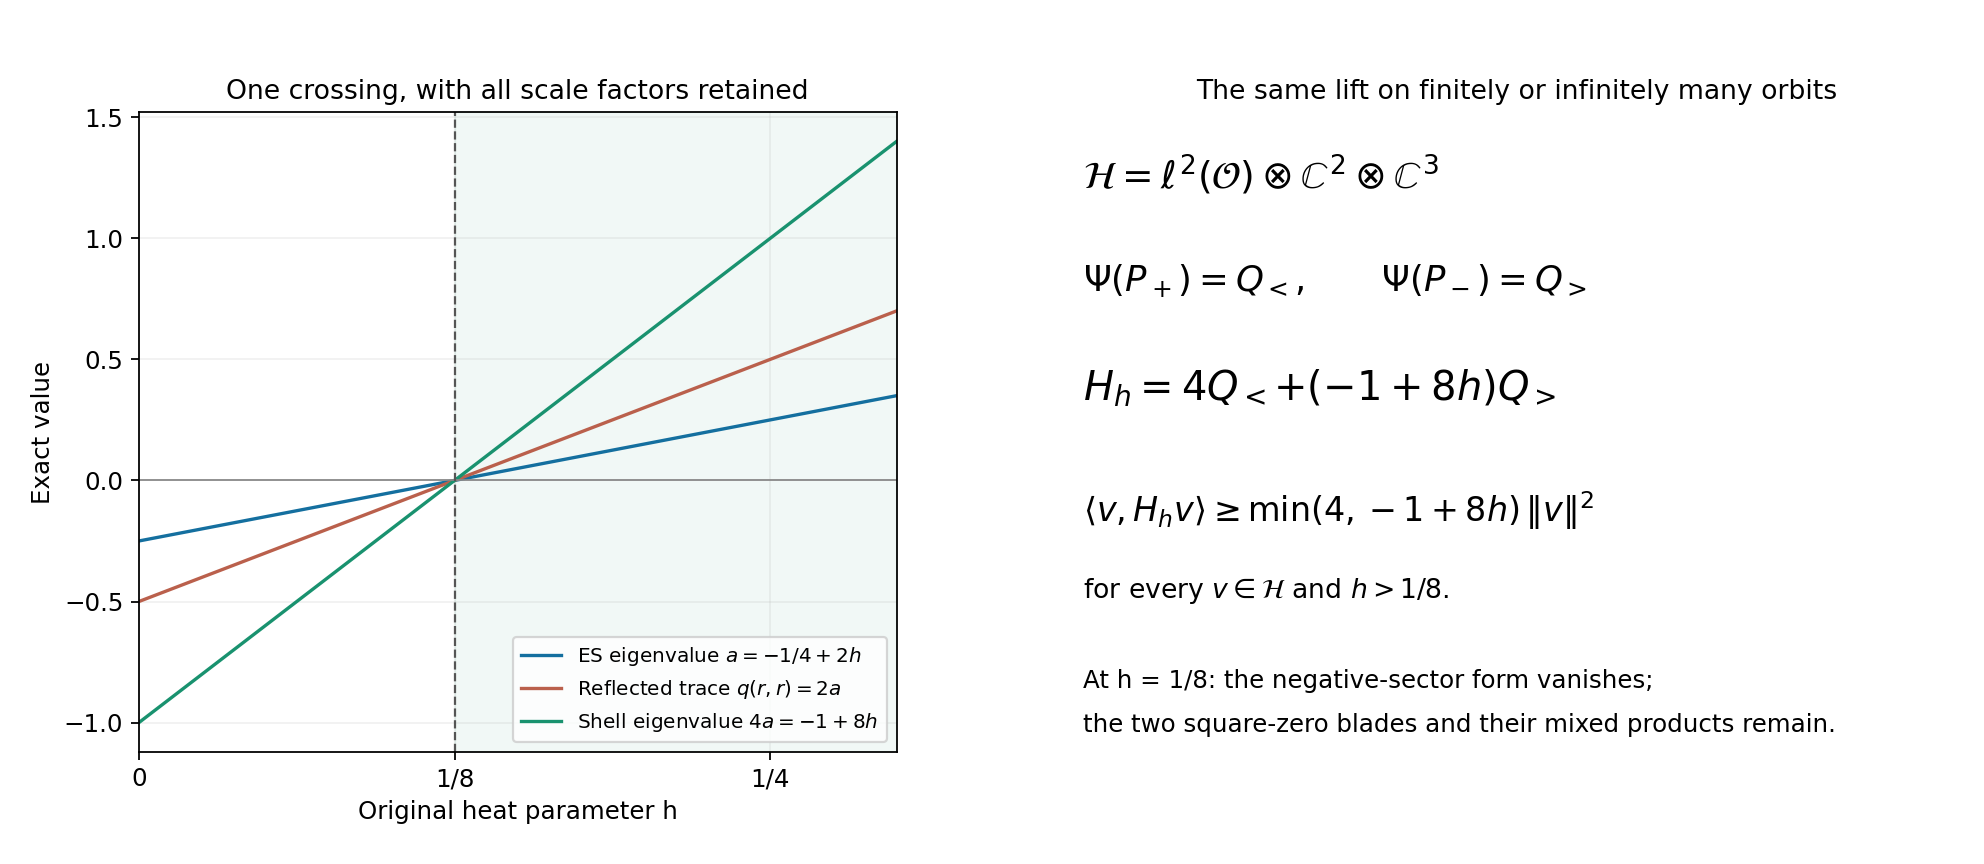
\includegraphics[keepaspectratio,alt={The three exact changing coefficients and their common crossing. The quarter coefficient is a, its reflected trace is 2a, and the shell coefficient is 4a. ESHL12--ESHL25 and ESHL34--ESHL42 prove the finite and infinite maps, sharp bound, surviving blades and trace scope.}]{figures/28_shell_heat_sign.png}}
\caption{The three exact changing coefficients and their common
crossing. The quarter coefficient is a, its reflected trace is 2a, and
the shell coefficient is 4a. ESHL12--ESHL25 and ESHL34--ESHL42 prove the
finite and infinite maps, sharp bound, surviving blades and trace
scope.}
\end{figure}

\end{document}
